% ===================================================================== PARTE IV
\chapter{Herramientas de software}

\begin{longtable}{p{0.2\textwidth}p{0.74\textwidth}}
\toprule
\textbf{Herramienta} & \textbf{Qué es y para qué se usa aquí} \\
\midrule
\endhead
Python 3.12 & El lenguaje del proyecto. Las librerías científicas hacen el trabajo
pesado: \textbf{NumPy} (vectores y matrices), \textbf{SciPy} (valores propios, matrices
dispersas, estadística), \textbf{pandas} (tablas), \textbf{NetworkX} (grafos),
\textbf{scikit-learn} y \textbf{XGBoost} (aprendizaje automático), \textbf{PyTorch} y
\textbf{PyTorch Geometric} (GCN y PINN), \textbf{SHAP} (explicaciones),
\textbf{Plotly} y \textbf{Matplotlib} (gráficas). \\
uv & Gestor de entornos y dependencias (como \texttt{pip} + \texttt{venv}, más rápido).
\texttt{uv sync} instala exactamente las versiones de \texttt{uv.lock}; \texttt{uv run}
ejecuta dentro de ese entorno. \\
\texttt{pyproject.toml} & Ficha del proyecto: nombre, versión, dependencias, comando
\texttt{pulso} y configuración de las herramientas. \\
YAML & Formato de texto para configuración (como un diccionario de Python en un
archivo). Cada experimento queda documentado con sus parámetros exactos. \\
Parquet & Formato de tabla en archivo: como CSV, pero comprimido, rápido y con tipos
fijos. \texttt{pd.read\_parquet} lo lee. \\
pytest & Corre las pruebas: funciones \texttt{test\_...} que verifican resultados. \\
ruff & Revisa el estilo y errores comunes sin ejecutar el código, y lo formatea. \\
git & Historial de versiones. Cada fase se trabajó en una \emph{rama} y se unió a
\texttt{main} solo con las pruebas en verde. \\
Streamlit & Convierte scripts de Python en una aplicación web interactiva. \\
Docker & Empaqueta Python, librerías, código, datos y modelos en una \emph{imagen} que
corre igual en cualquier computador. \\
GitHub Actions & Integración continua: en cada cambio subido corre ruff, pytest y
construye la imagen Docker. \\
LaTeX & Con el que se escribió esta guía y la presentación. \\
\bottomrule
\end{longtable}

% ---------------------------------------------------------------------------
\chapter{Instalación y ejecución}

\section{Instalación}
\begin{enumerate}
\item Instalar \texttt{uv} (\url{https://docs.astral.sh/uv/}).
\item En la carpeta del proyecto:
\begin{codigo}[label=terminal]
uv sync                      # crea el entorno e instala todo
uv run pytest -m "not slow"  # pruebas rápidas (~10 s)
uv run pytest                # todas las pruebas (~1 min)
\end{codigo}
\end{enumerate}

\section{La aplicación}
\begin{codigo}[label=terminal]
uv run streamlit run app/Inicio.py      # abre http://localhost:8501
\end{codigo}
Si el puerto 8501 está ocupado: \texttt{--server.port=8502}.

\section{Comandos del proyecto}
\begin{codigo}[label=terminal]
uv run pulso sweep  configs/sweep.yaml    # dataset de la tarea 5 (~20 min, 8 núcleos)
uv run pulso train  configs/train.yaml    # modelos de la tarea 5
uv run pulso world  configs/world.yaml    # un mundo multicapa -> data/world/demo
uv run pulso credit configs/credit.yaml   # experimento y modelos de la tarea 6 (~20 s)
uv run pulso --help                       # ayuda
\end{codigo}

\section{Con Docker}
\begin{codigo}[label=terminal]
docker build -t pulso .
docker run -p 8501:8501 pulso
\end{codigo}
La imagen incluye los datos y modelos ya entrenados: la app funciona sin correr
ningún experimento.

\section{Regenerar esta documentación}
\begin{codigo}[label=terminal]
PYTHONPATH=src uv run python docs/latex/figuras.py   # figuras de la tarea 6
bash docs/latex/compilar.sh                          # todos los PDF -> docs/Presentaciones/
\end{codigo}

\section{Modificación de parámetros}
Ejemplo: evaluar un acoplamiento de nómina más intenso. Se edita
\archivo{configs/credit.yaml}:
\begin{codigo}[label=configs/credit.yaml]
dynamics:
  alpha: 1.0                       # 1/mes: el déficit se corrige en ~1 mes
  beta: {N: 0.5, S: 0.4, T: 0.3}   # amplificación del déficit de quien paga
  K: {N: 0.8, S: 1.0, T: 0.3}      # ajuste del ritmo al de los pagadores
  gamma: 0.5                       # ingreso desfasado que se vuelve déficit
  loss: 1.0                        # perder un pagador del 100 % del ingreso
  noise: 0.3                       # choques idiosincráticos de liquidez
\end{codigo}
y se vuelve a correr \texttt{uv run pulso credit configs/credit.yaml}. No se toca el
código.

% ---------------------------------------------------------------------------
\chapter{La aplicación web}

\begin{figure}[h]
\centering
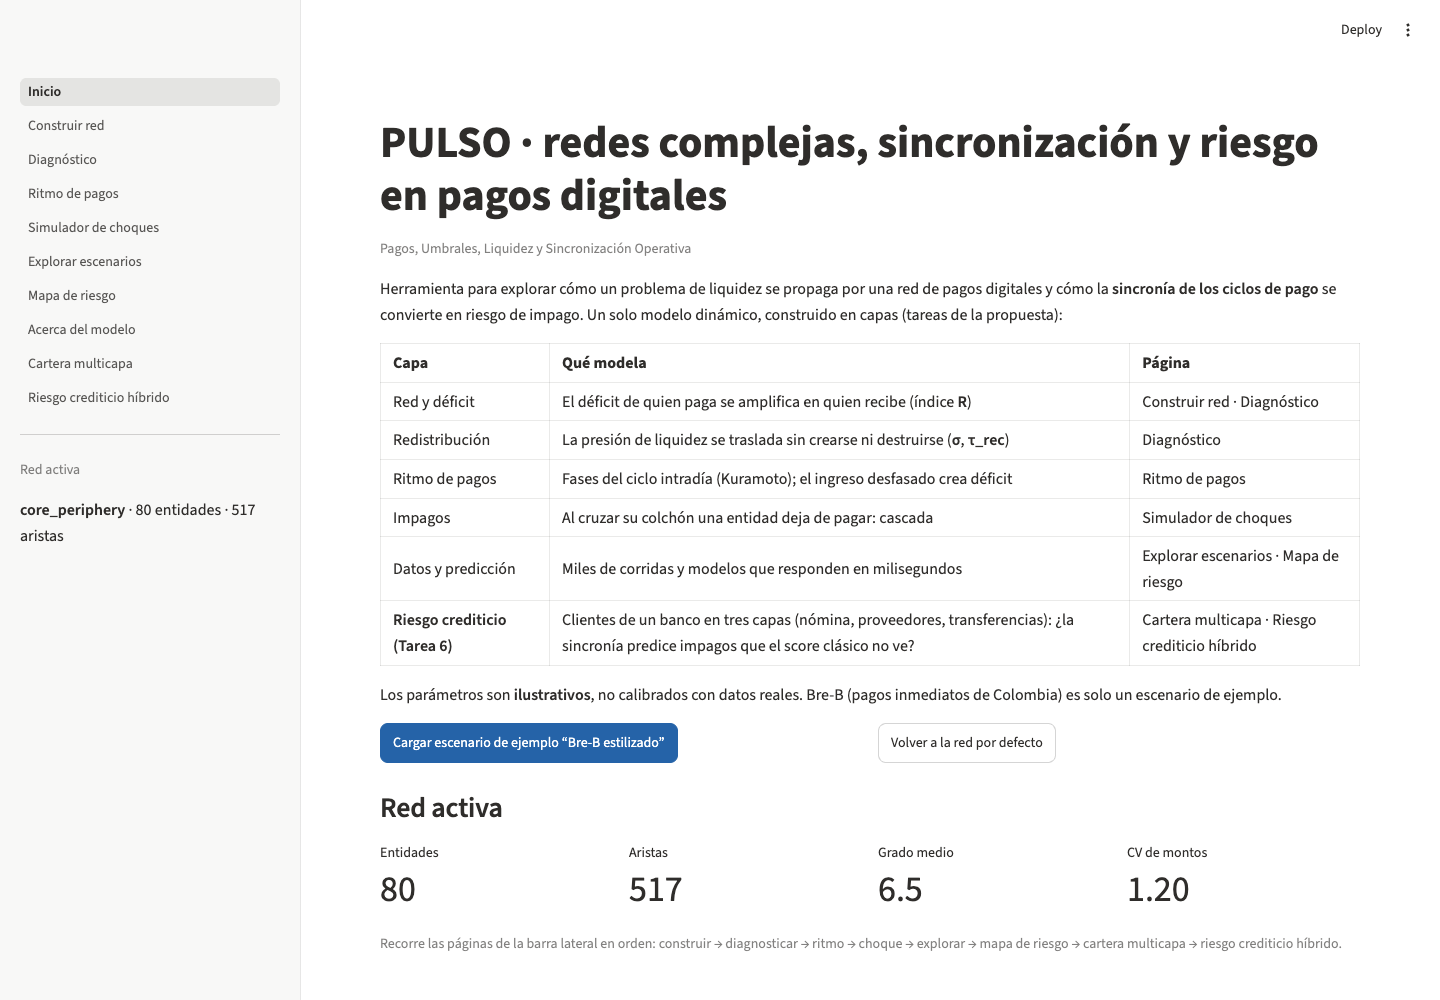
\includegraphics[width=0.92\textwidth]{app_inicio.png}
\caption{Inicio: el resumen de las capas del modelo y la red activa. El botón carga el
escenario de ejemplo ``Bre-B estilizado'' (núcleo-periferia, 245 entidades).}
\end{figure}

\begin{description}
\item[Construir red.] Se elige topología, tamaño, grado medio y dispersión de montos.
\item[Diagnóstico.] $R$, estabilidad $\sigma$ con semáforo, tiempo de recuperación,
$\lambda_2$, comunidades y ranking de entidades por importancia y vulnerabilidad.
\item[Ritmo de pagos.] $K$, dispersión de ritmos, $\gamma$; círculo de fases animado,
$r(t)$ y déficit; se puede desconectar una entidad a mitad de la corrida.
\item[Simulador de choques.] Se elige entidad y tipo de choque; cascada animada,
porcentaje en impago, liquidez no pagada, DebtRank y línea de tiempo de eventos.
\item[Explorar escenarios.] El dataset de 20\,000 escenarios: dónde colapsa la red.
\item[Mapa de riesgo.] Predicción instantánea por entidad (GCN, XGBoost), explicación
SHAP y botón ``verificar con simulación''.
\item[Acerca del modelo.] Ecuaciones, supuestos y límites.
\item[Cartera multicapa.] Tarea 6: la cartera del banco, sus capas, la sincronía
global estimada contra la real, impago según sincronía y el escenario de quiebra de
un empleador.
\item[Riesgo crediticio híbrido.] Tarea 6: la comparación de los tres niveles con su
control, la PD por cliente (clásica contra híbrida), los clientes con ``riesgo
oculto'' y la explicación SHAP de cada predicción.
\end{description}

\begin{figure}[p]
\centering
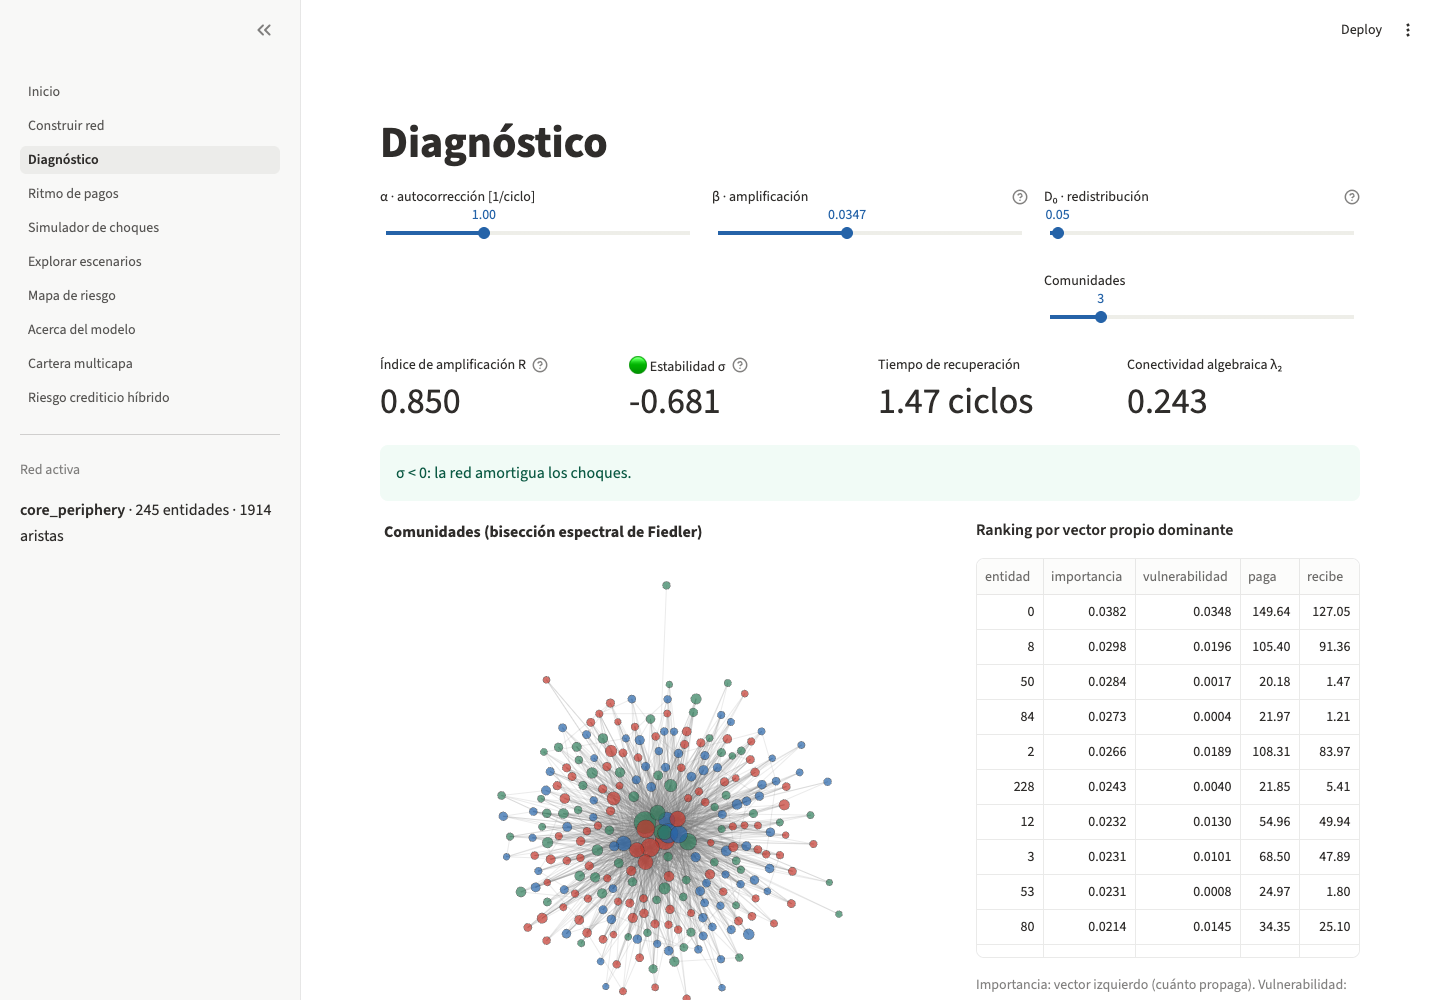
\includegraphics[width=0.49\textwidth]{app_diagnostico.png}\hfill
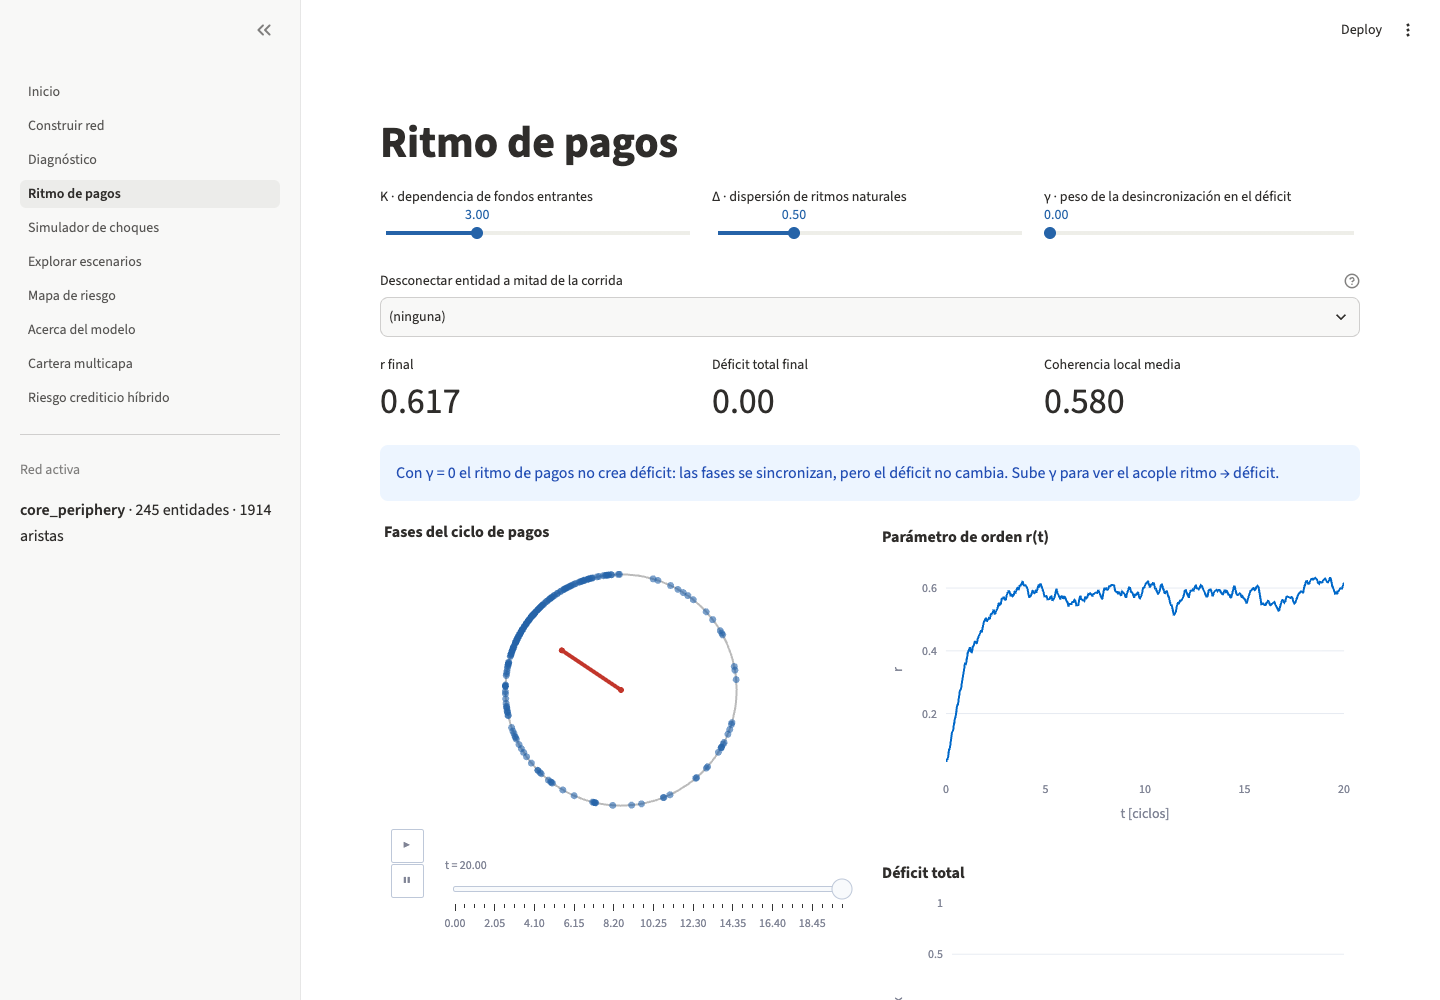
\includegraphics[width=0.49\textwidth]{app_ritmo.png}\\[4pt]
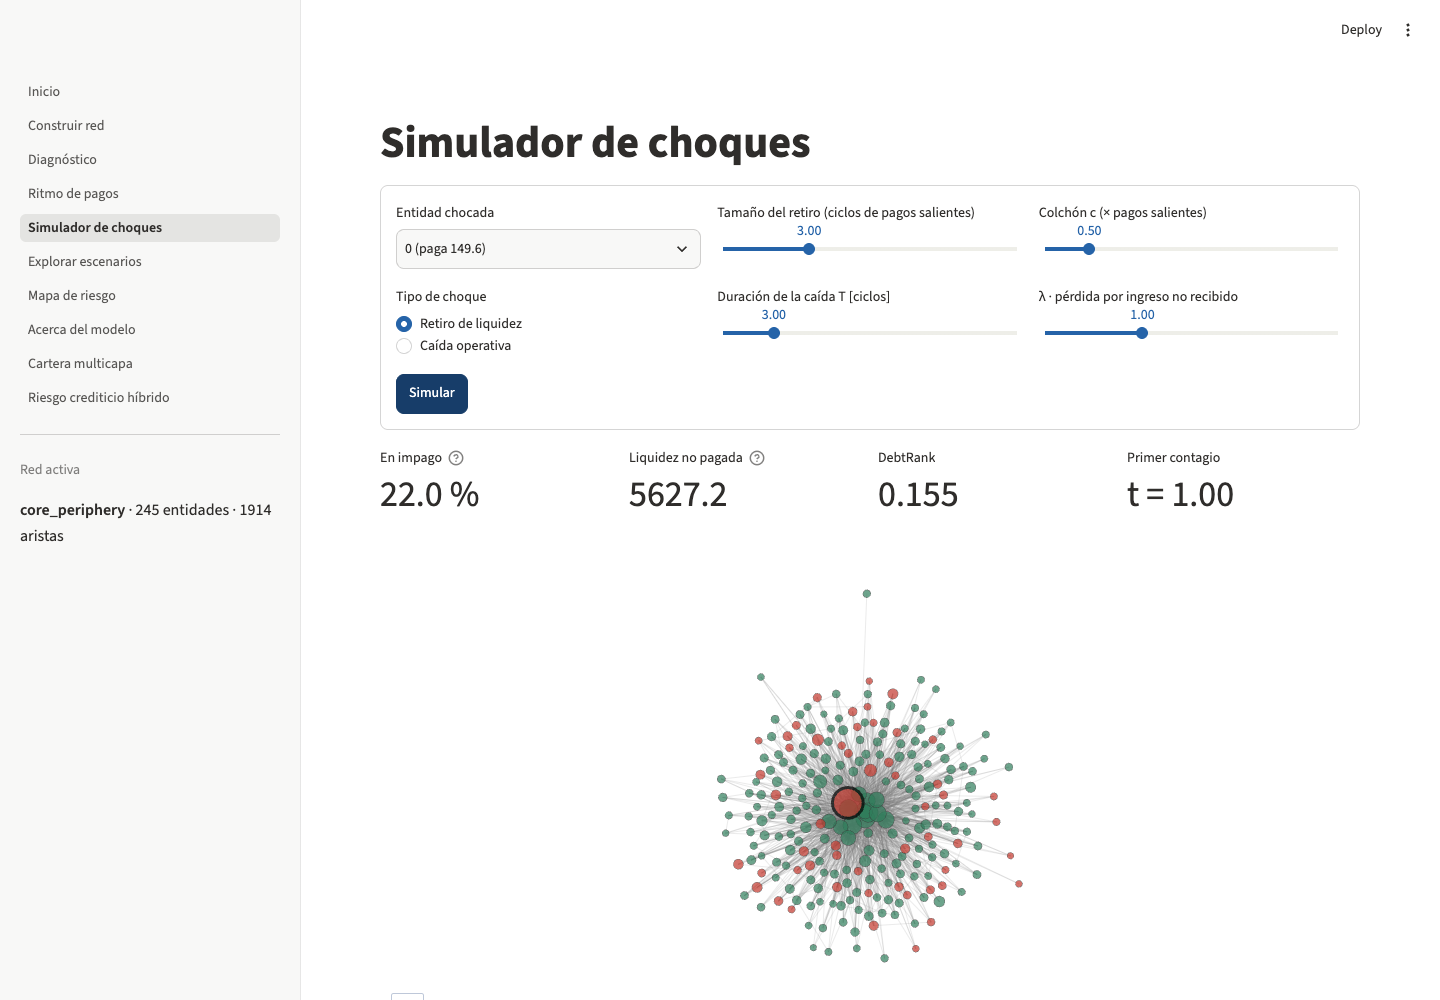
\includegraphics[width=0.49\textwidth]{app_simulador.png}\hfill
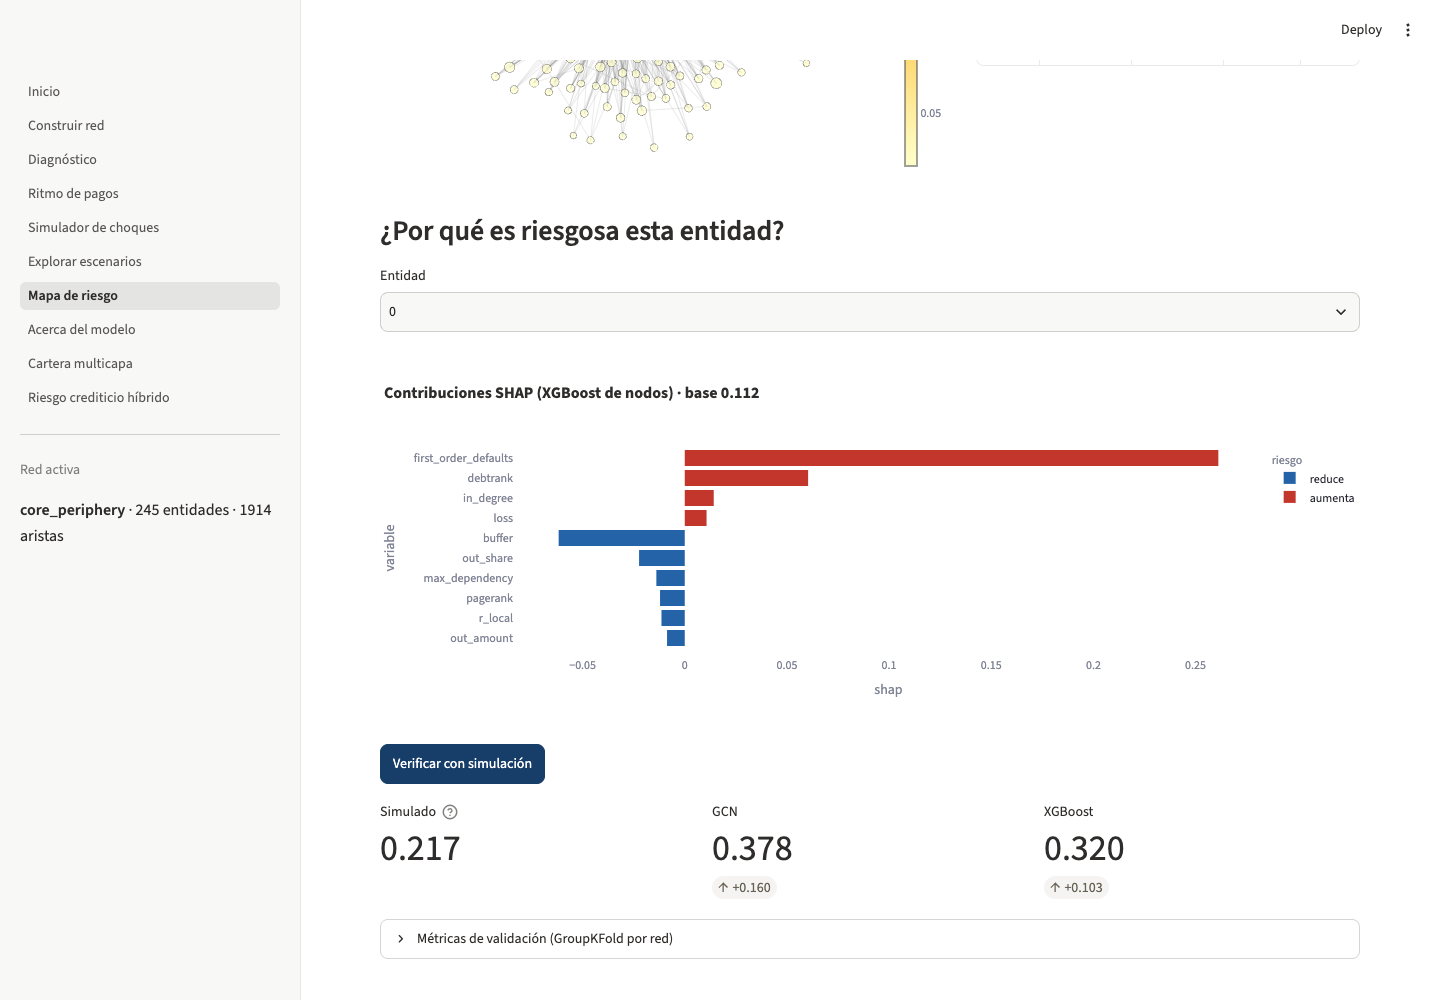
\includegraphics[width=0.49\textwidth]{app_mapa.png}
\caption{Diagnóstico, Ritmo de pagos, Simulador de choques y Mapa de riesgo.}
\end{figure}

\begin{figure}[p]
\centering
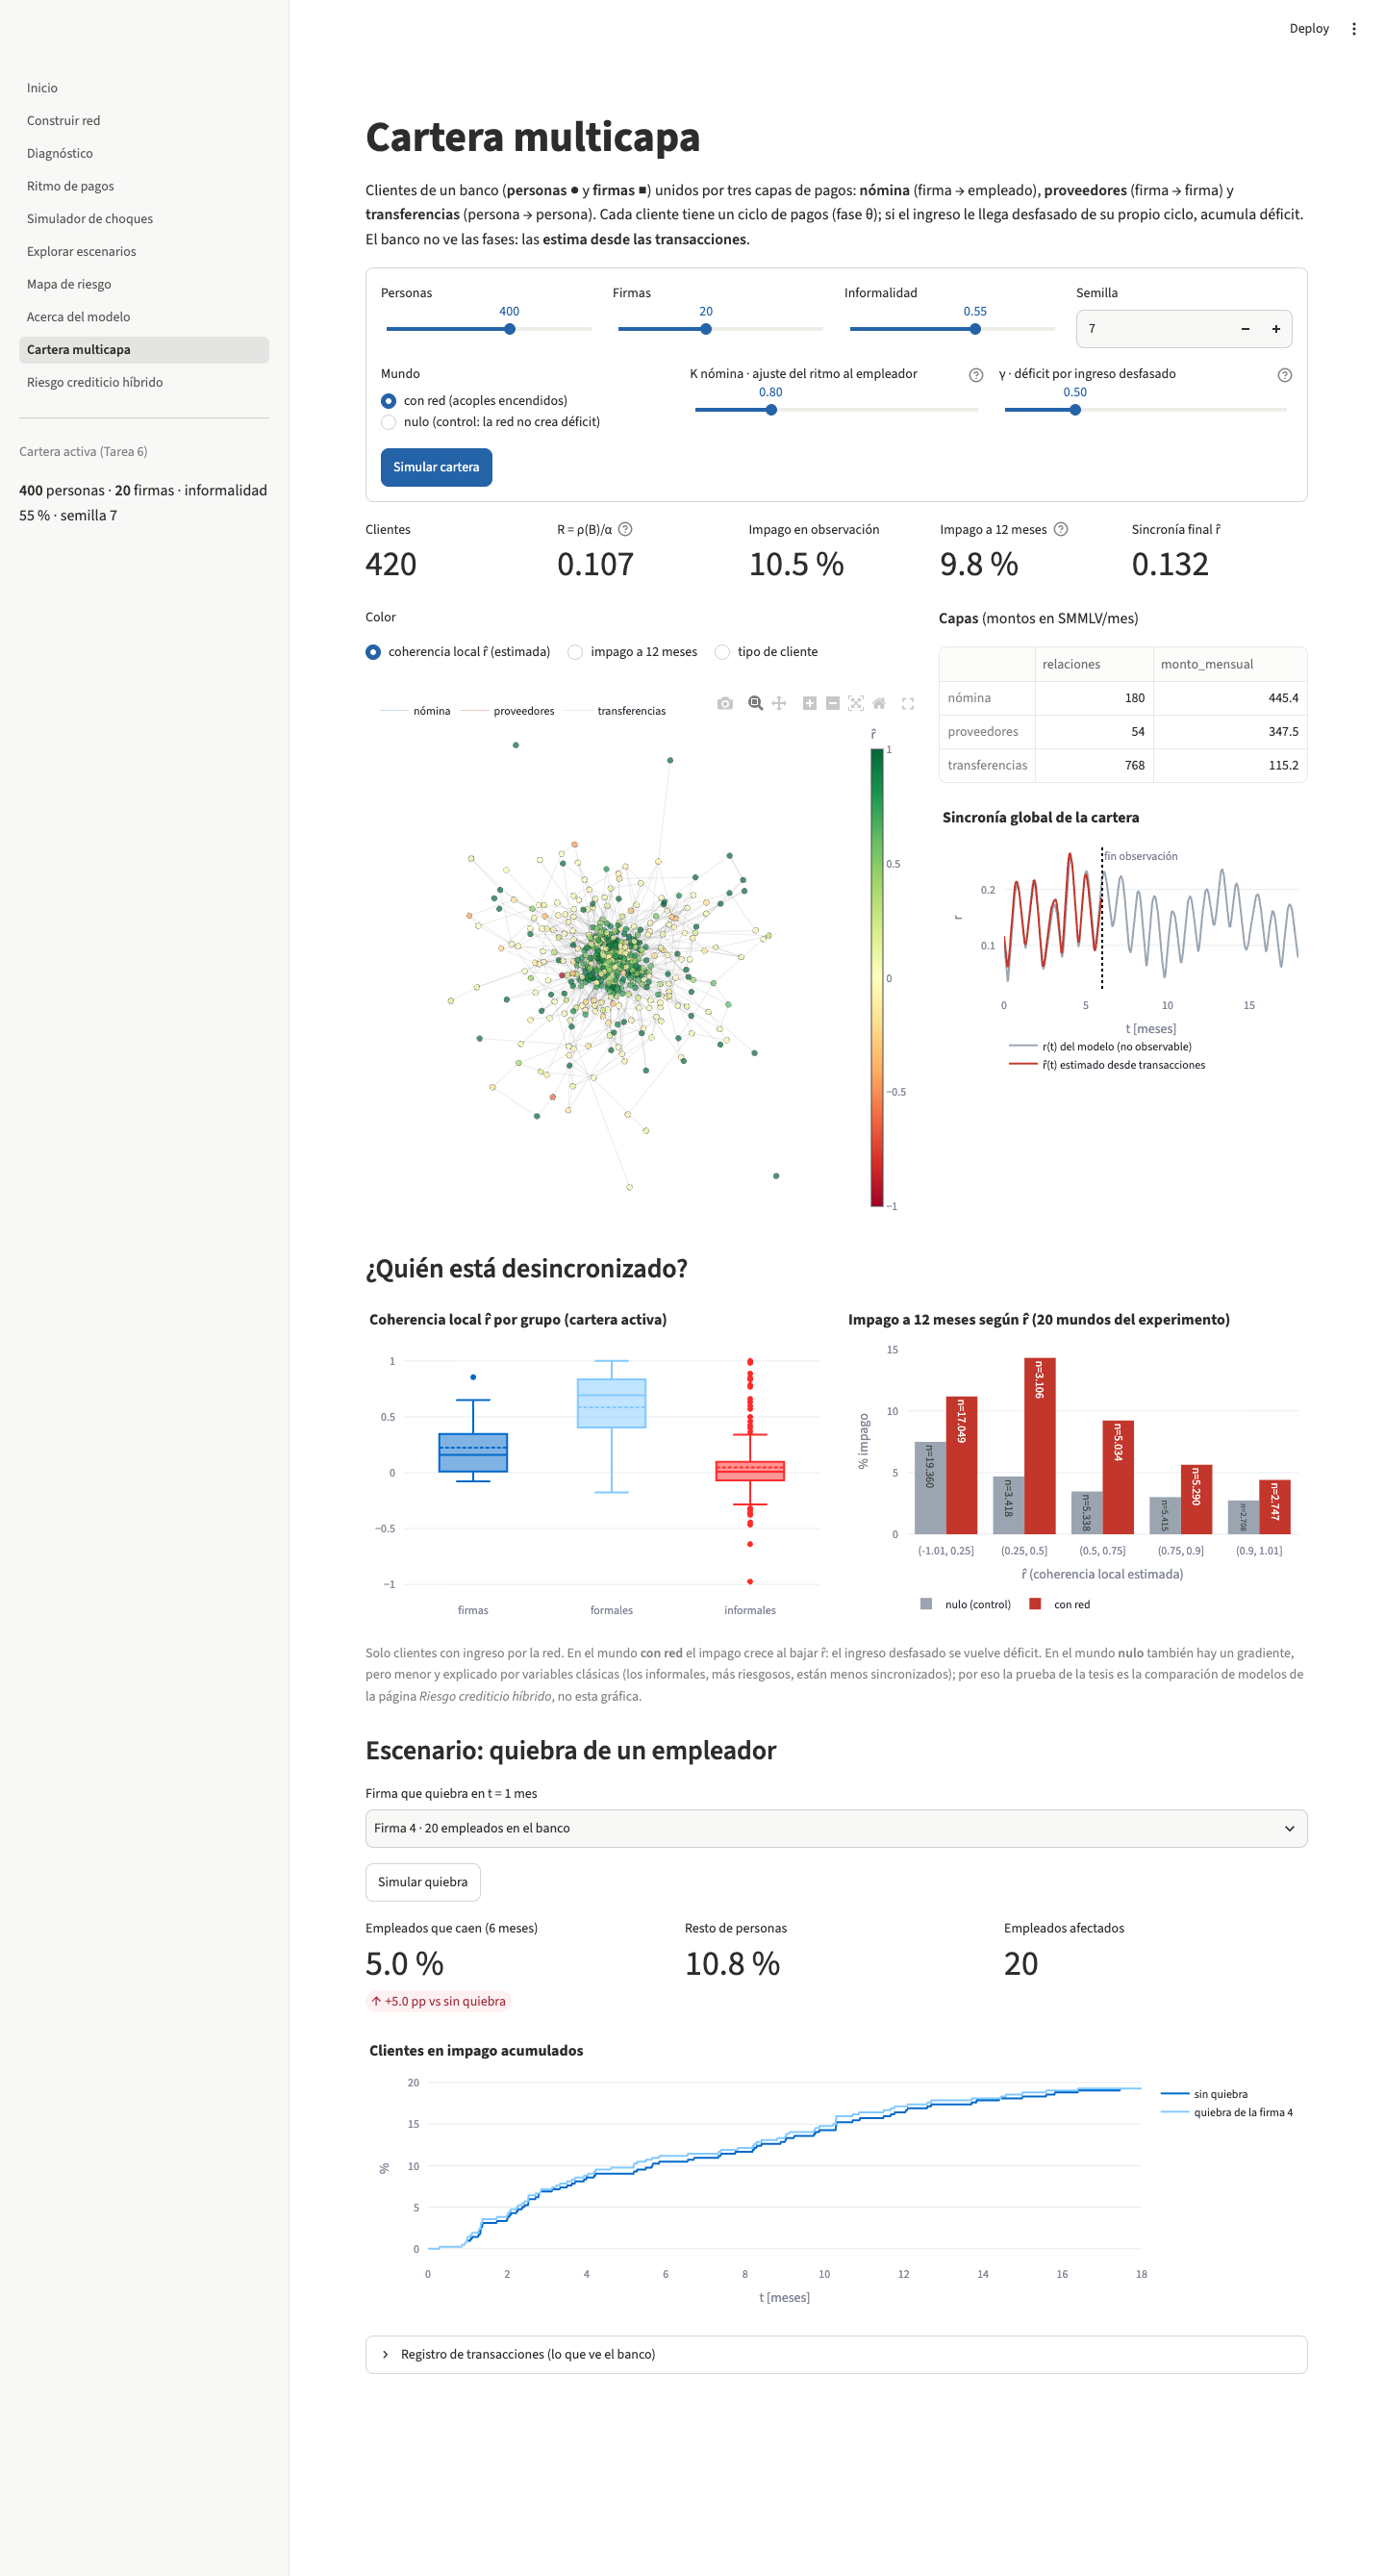
\includegraphics[height=0.86\textheight]{app_cartera_completa.png}
\caption{Cartera multicapa, con el escenario de quiebra simulado.}
\end{figure}

\begin{figure}[p]
\centering
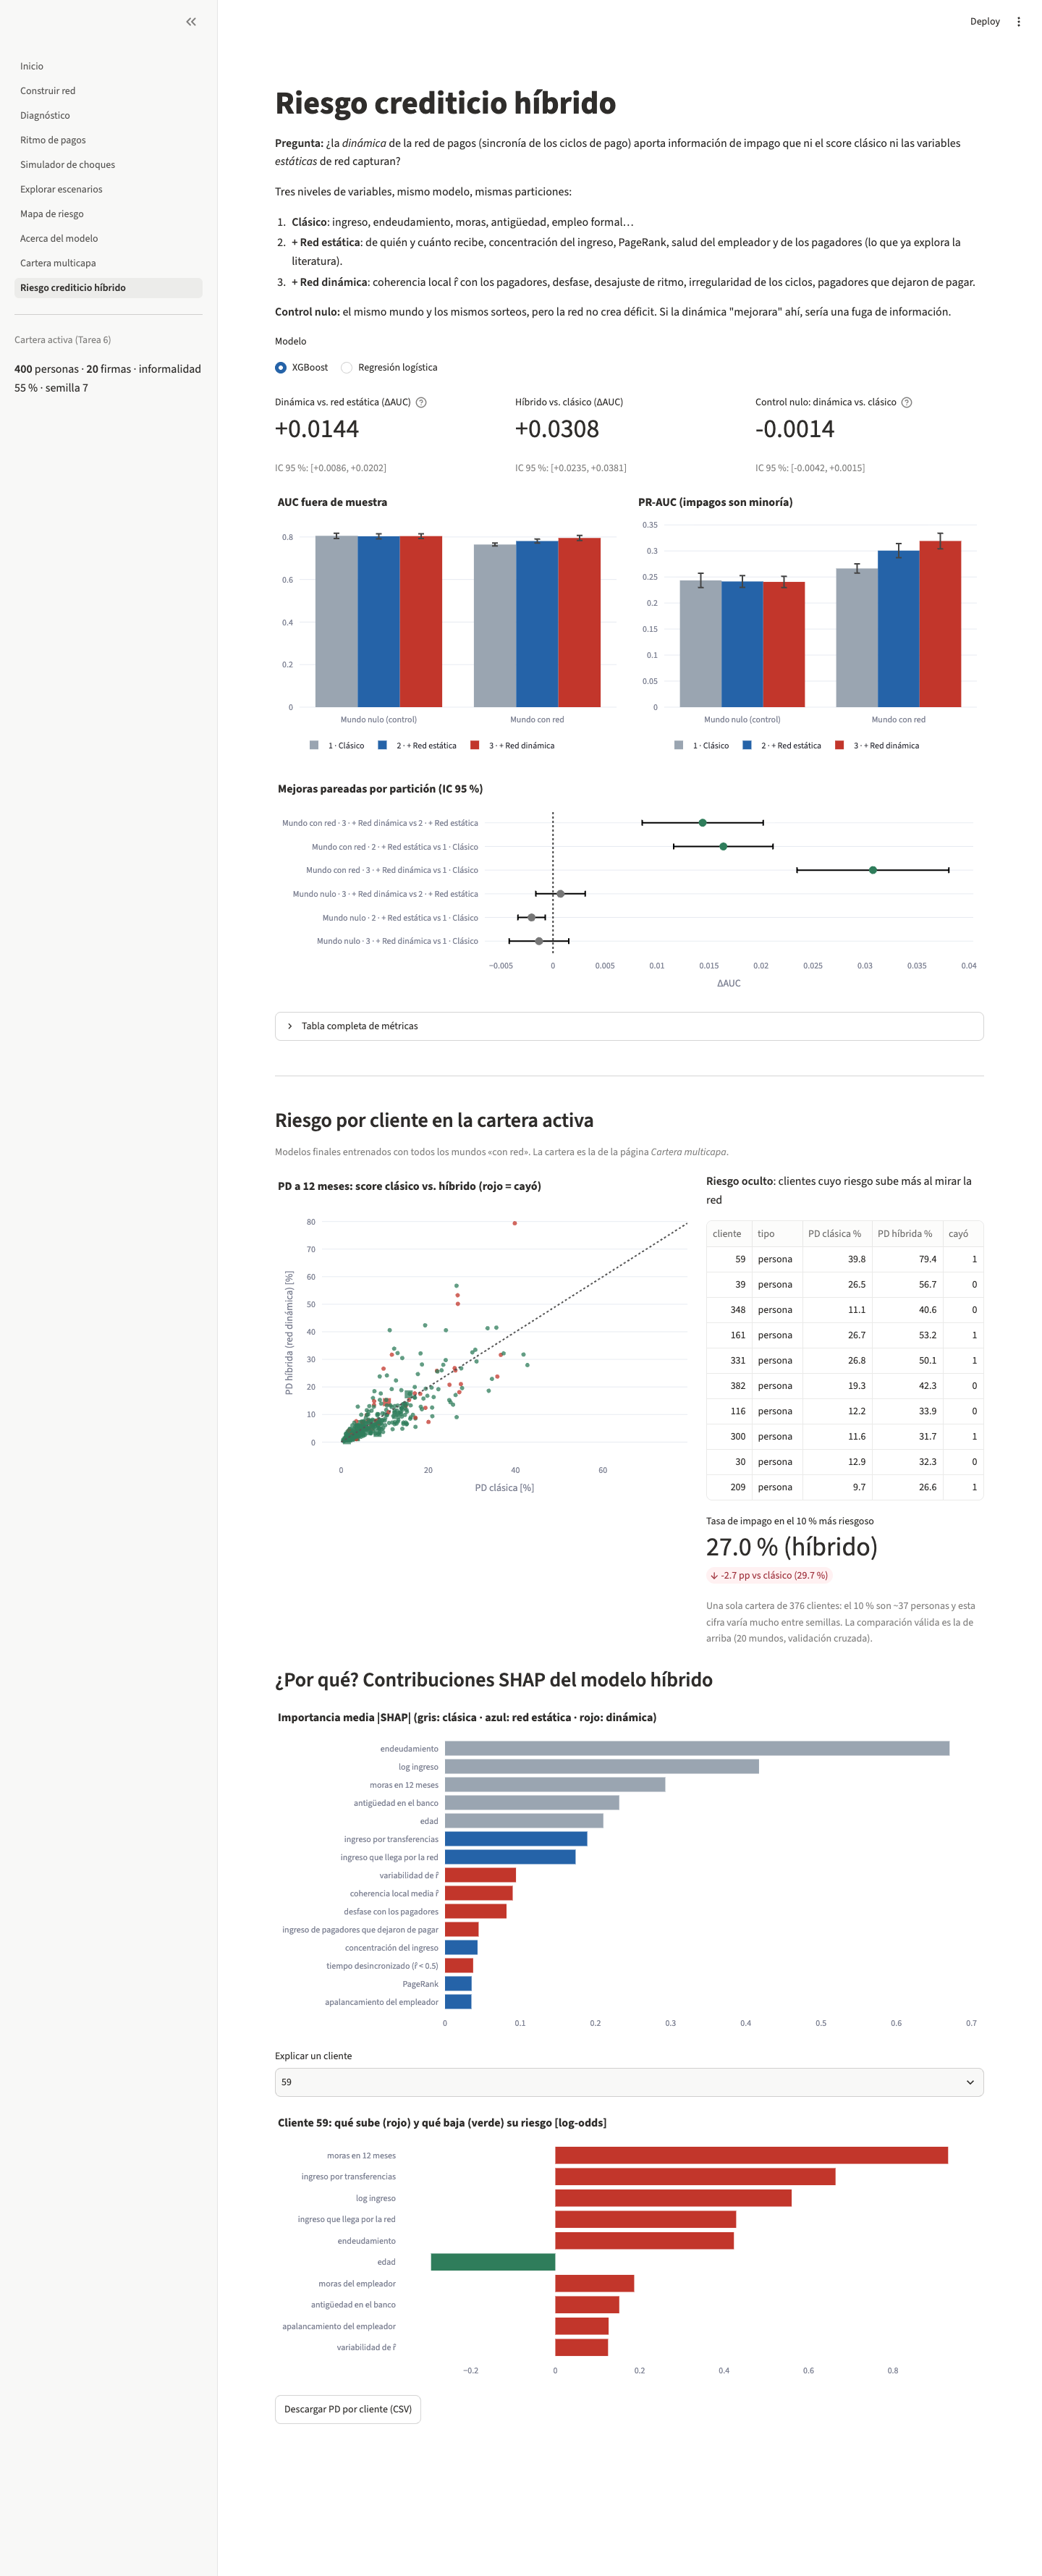
\includegraphics[height=0.86\textheight]{app_hibrido_completa.png}
\caption{Riesgo crediticio híbrido.}
\end{figure}

% ---------------------------------------------------------------------------
\chapter{Organización del proyecto}

\begin{codigo}[label=estructura de carpetas]
pulso/
├── README.md, CHANGELOG.md        qué es, cómo usarlo, historial de versiones
├── pyproject.toml, uv.lock        dependencias exactas
├── Dockerfile, .dockerignore      imagen de la app
├── .github/workflows/ci.yml       pruebas y Docker en cada cambio
├── configs/                       TODOS los parámetros (YAML)
│   ├── default.yaml, breb_example.yaml       app, tareas 1–4
│   ├── sweep.yaml, train.yaml, pinn.yaml     tarea 5
│   └── world.yaml, credit.yaml               tarea 6
├── src/pulso/                    el núcleo (paquete de Python)
│   ├── networks, model, integrate, spectral, cascades, metrics
│   ├── experiments, ml/            tarea 5
│   ├── world/, credit/             tarea 6
│   ├── service.py, schema.py, config.py, cli.py, viz.py
├── app/                           Inicio.py, common.py, pages/1..9
├── tests/                         test_fase1..6, test_fase10..12, test_app
├── notebooks/                     01..06: exploración y figuras por tarea
├── data/                          datasets (tarea 5) y data/credit/ (tarea 6)
├── models/                        modelos versionados; models/credit/v1
├── figures/                       figuras de las tareas 1–6
└── docs/
    ├── Presentaciones/
    │   ├── v1/                    esta guía y la presentación completa
    │   └── v2/                    presentación breve, guion y manual de la app
    ├── bibliografia.md
    ├── diseno/                    especificación de diseño de la tarea 6
    └── latex/                     fuentes de los PDF, figuras y compilar.sh
\end{codigo}

Archivos que \emph{no} se guardan en git porque se regeneran: el entorno
(\texttt{.venv/}), las cachés (\texttt{\_\_pycache\_\_}, \texttt{.pytest\_cache},
\texttt{.ruff\_cache}), los temporales (\texttt{data/tmp/}) y la tabla grande de
clientes de la tarea 6 (\texttt{data/credit/clientes.parquet}, se rehace en segundos).

% ---------------------------------------------------------------------------
\chapter{Problemas conocidos y trabajo futuro}

\section{Problemas conocidos (macOS)}
\begin{itemize}
\item \texttt{ModuleNotFoundError: No module named 'pulso'} dentro de
\texttt{\textasciitilde/Documents}: macOS oculta el archivo \texttt{.pth} de la
instalación editable. Solución: \texttt{chflags -R nohidden .venv}, o anteponer
\texttt{PYTHONPATH=src}.
\item torch y xgboost traen cada uno su propia librería OpenMP; el proyecto carga
xgboost primero y deja torch en un hilo para evitar cierres inesperados.
\end{itemize}

\section{Trabajo futuro}
\begin{enumerate}
\item \textbf{Datos reales}: correr el pipeline de la tarea 6 sobre una cartera
anonimizada. Es el paso que convierte el mecanismo en evidencia.
\item \textbf{Revisión bibliográfica sistemática} (Scopus, Web of Science) sobre
sincronización y riesgo de crédito.
\item \textbf{Fecha de cuota y plazos} como forzamiento externo del ritmo.
\item \textbf{Retroalimentación}: que el déficit también cambie el ritmo de pago.
\item \textbf{Observabilidad parcial}: un banco solo ve a sus clientes; el operador de
un sistema interoperable como Bre-B ve la red completa.
\end{enumerate}
